\documentclass{article}
\usepackage[utf8]{inputenc}
\usepackage{ctex}
\usepackage{amsmath}
\usepackage{float}
\usepackage{natbib}
% \usepackage{csvsimple}
\usepackage{tabularx}
\usepackage{booktabs}
\usepackage{longtable}
\usepackage{graphicx}
\graphicspath{{E:/Github/CourseWork/StochasticProcess/figs/}}


\title{随机过程大作业}
\author{张栩萌 \ 519070910031}
\date{May 2022}



\begin{document}

\maketitle

\section{实验目的}
1. 通过计算机模拟布朗运动,观察布朗运动的特性

2. 通过计算机模拟随机微分方程解的轨道,探究不同参数对轨道的影响,计算机模拟$X_1$的期望和方差

3. 熟练Python编程建模操作




\section{问题一:布朗运动}
布朗运动的定义为:若一个随机过程$\{X(t), t \ge 0\}$满足\\
$X(t)$ 是独立增量过程;\\
$\forall s, t>0, X(s+t)-X(s) \sim N\left(0, c^{2} t\right)$, 即 $X(t+s)-X(s)$ 是数学期望 为 0 , 方差为 $c^{2} t$ 的正态分布;\\
$X(t)$ 关于 $t$ 是连续函数,\\
则称 $\{X(t), t \ge 0\}$ 是布朗运动或维纳过程. 当 $c=1$ 时, 称 $\{X(t), t \ge 0\}$ 是标准布朗运动。

图\ref{fig:brown1}为在$[0, 1]$区间生成100个等距点,以0.1为时间间隔生成的标准布朗运动,图\ref{fig:brown1_10}为同样的区间节点下生成的$c=10$时的布朗运动。

\begin{figure}[H]
    \centering
    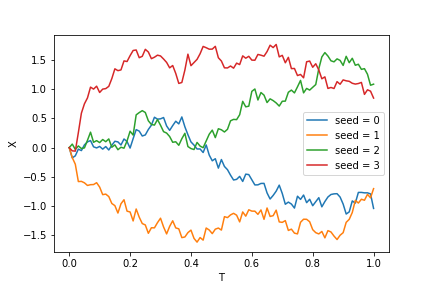
\includegraphics[scale=.6]{多条布朗运动轨道.png}
    \caption{多条标准布朗运动轨道}
    \label{fig:brown1}
    \end{figure}

\begin{figure}[H]
    \centering
    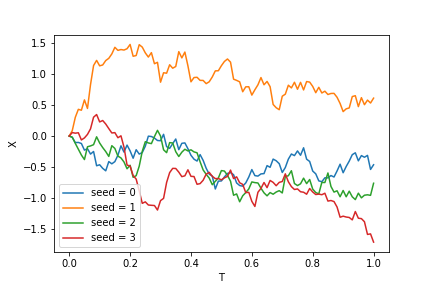
\includegraphics[scale=.6]{多条布朗运动轨道c=10.png}
    \caption{当$c=10$时多条布朗运动轨道}
    \label{fig:brown1_10}
    \end{figure}

因为参数$c$影响布朗运动的增量正态分布的方差,所以我们看到当$c=10$时布朗运动振荡的幅度明显大于标准布朗运动。




\section{问题二:股票价值随机微分方程}
设 $B=\left\{B_{t} ; t \geq 0\right\}$ 为标准布朗运动, $X=\left\{X_{t} ; t \geq 0\right\}$ 为如下随机微分方程的解:
$$
\left\{\begin{array}{l}
d X_{t}=\alpha\left(v-X_{t}\right) d t+\sigma d B_{t} \\
X_{0}=x_{0}
\end{array}\right.
$$
其中 $\alpha, v, \sigma, x_{0}$ 为常数。


接下来我们测试不同参数对轨道的作用。

在微分方程中,$d B_t$ 是一个正态的扰动,前面的方程 $d X_{t}=\alpha\left(v-X_{t}\right) d t$ 表示了如果 $X_t$ 不等于 $v$ 的话,$X_t$ 会以一定速度向 $v$ 收敛。如果把 $X_t$ 看作是函数的话这个微分方程的函数解是 $f = \frac{1}{\alpha} exp{-\alpha t} + v + C$ 所以$v$代表了$X_t$的稳态。而$\alpha$就代表了收敛的速度。下面的实验对这些分析进行了验证


\begin{figure}[H]
    \centering
    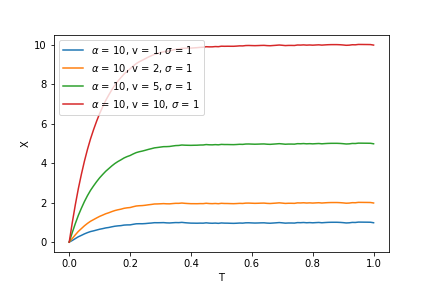
\includegraphics[scale=.6]{随机微分方程解1参数v.png}
    \caption{参数 $v$ 对随机微分方程1解的轨道影响}
    \label{fig:SDE1_v}
    \end{figure}



\begin{figure}[H]
    \centering
    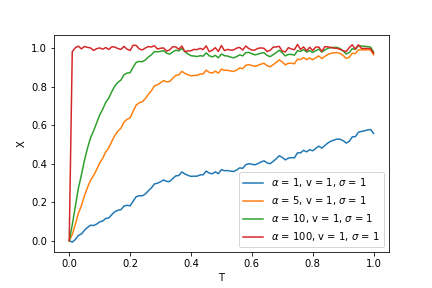
\includegraphics[scale=.6]{随机微分方程解1参数alpha.png}
    \caption{参数 $\alpha$ 对随机微分方程1解的轨道影响}
    \label{fig:SDE1_alpha}
    \end{figure}





\begin{figure}[H]
    \centering
    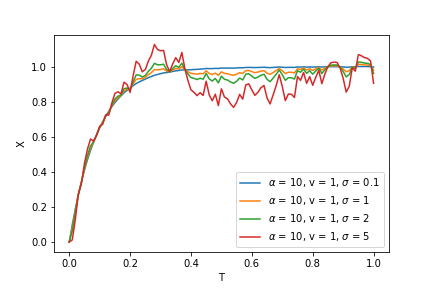
\includegraphics[scale=.6]{随机微分方程解1参数sigma.png}
    \caption{参数 $\sigma$ 对随机微分方程1解的轨道影响}
    \label{fig:SDE1_sigma}
    \end{figure}


\begin{figure}[H]
    \centering
    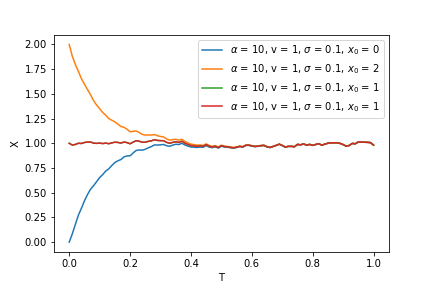
\includegraphics[scale=.6]{随机微分方程解1参数x0.png}
    \caption{参数 $x_0$ 对随机微分方程1解的轨道影响}
    \label{fig:SDE1_x0}
    \end{figure}


图\ref{fig:SDE1_alpha}说明$\alpha$ 越大收敛的速度越快;图\ref{fig:SDE1_sigma}说明$\sigma$ 越大噪声的振荡越大;图\ref{fig:SDE1_alpha}和图\ref{fig:SDE1_alpha}说明$v$ 决定$X_t$最终的稳态,而$x_0$决定$X_t$的初态。

我们现在用Monte-Carlo模拟查看不同参数下$X_t$稳态分布的期望与方差。下面的实验都是在控制单一变量的条件下进行的,控制的变量默认为 $\alpha = 10, \ v=1,\ \sigma=1 , \ x_0 = 0$。

\begin{table}[H]
    \centering
    \caption{不同参数下的 $E(X_1)$ 和 $D(X_1)$}
    \begin{tabular}{l|l|l|l|l|l}
    \hline
    $\alpha$ & $E(X_1)$ & $D(X_1)$ & $v$    & $E(X_1)$ & $D(X_1)$ \\ \hline
    1     & 0.636873 & 0.004301 & 1    & 1.000939  & 0.000513 \\
    2     & 0.869714 & 0.002371 & 2    & 2.000912  & 0.000513 \\
    5     & 0.99551  & 0.000966 & 5    & 5.000832  & 0.000513 \\
    10    & 1.000939 & 0.000513 & 10   & 10.000699 & 0.000513 \\ \hline 
    $\sigma$ & $E(X_1)$ & $D(X_1)$ & $x_0$ & $E(X_1)$ & $D(X_1)$ \\ \hline
    0.1   & 1.00007  & 5e-06    & 0    & 1.000939  & 0.000513 \\
    1.0   & 1.000939 & 0.000513 & 2    & 1.000992  & 0.000513 \\
    2.0   & 1.001904 & 0.00205  & 5    & 1.001071  & 0.000513 \\
    5.0   & 1.004799 & 0.012815 & 10   & 1.001204  & 0.000513 \\ \hline
    \end{tabular}
\end{table}
    
实验结果表明,$v$与$E(X_1)$正比,$\sigma$的平方与$D(X_1)$正比,$\alpha$和$x_0$与这两个量无关。




\section{问题三:股票价值与价格随机微分方程}
设 $B=\left\{B_{t} ; t \geq 0\right\}$ 与 $W=\left\{W_{t} ; t \geq 0\right\}$ 为标准布朗运动, $X=\left(X_{t} , S_t\right)$ 为如下随机微分方程的解:
$$
\left\{\begin{array}{l}
d X_{t}=\alpha\left(v-X_{t}\right) d t+\sigma d B_{t} \\
d S_{t} = \alpha\left(X_{t}-S_{t}\right) d t+\hat{\sigma_1} dB_t + \hat{\sigma_2} dW_t\\
X_{0}=x_{0}, \ S_0 = s_0
\end{array}\right.
$$
其中 $\alpha, v, \sigma, \theta, \hat{\sigma_1}, \hat{\sigma_2}, x_{0}, s_0$ 为常数。

这个方程中可以将 $X_t$ 看作是股票价值,$S_t$ 看作是股票价格。当价格高于价值是,市场会对股票有一种看衰的期望;股票价格也将会随之下降,当价格低于价值时,市场就会对股票看好,价格也将随之上升。



\begin{figure}[H]
    \centering
    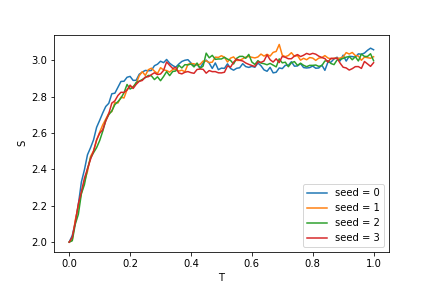
\includegraphics[scale=.6]{随机微分方程解2的多条轨道S-T.png}
    \caption{随机微分方程2解的多条轨道S-T}
    \label{fig:SDE2_S}
    \end{figure}

\begin{figure}[H]
    \centering
    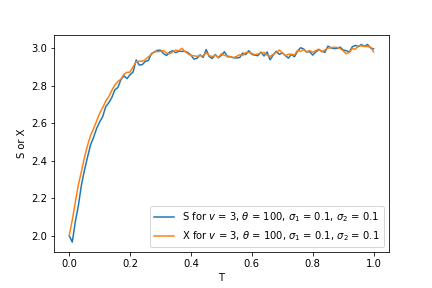
\includegraphics[scale=.6]{随机微分方程解2的多条轨道SX-T.png}
    \caption{随机微分方程2解的多条轨道S, X-T}
    \label{fig:SDE2_SX}
    \end{figure}


\begin{figure}[H]
    \centering
    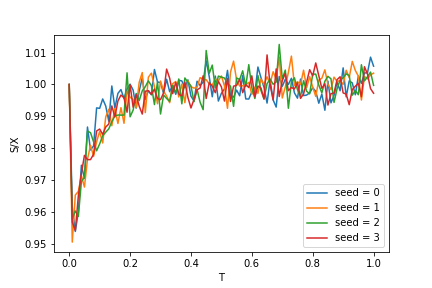
\includegraphics[scale=.6]{随机微分方程解2的多条轨道Ratio-T.png}
    \caption{随机微分方程2解的多条轨道S/X-T}
    \label{fig:SDE2_Ratio}
    \end{figure}

\begin{figure}[H]
    \centering
    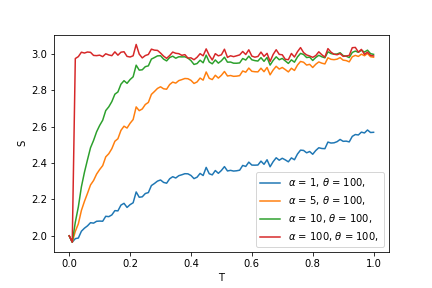
\includegraphics[scale=.6]{随机微分方程解2参数alpha.png}
    \caption{参数 $\alpha$ 对随机微分方程2解的轨道影响}
    \label{fig:SDE12_alpha}
    \end{figure}


\begin{figure}[H]
    \centering
    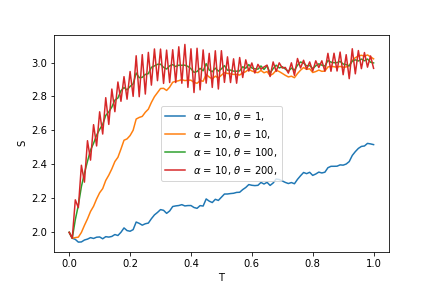
\includegraphics[scale=.6]{随机微分方程解2参数theta.png}
    \caption{参数 $\theta$ 对随机微分方程2解的轨道影响}
    \label{fig:SDE2_theta}
    \end{figure}



\begin{figure}[H]
    \centering
    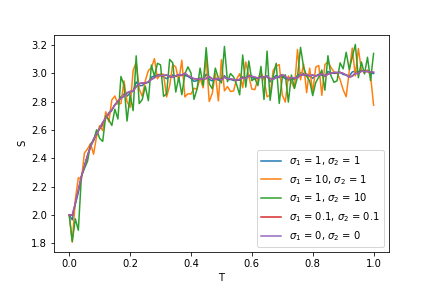
\includegraphics[scale=.6]{随机微分方程解2参数sigma.png}
    \caption{参数 $\sigma$, $\sigma_1$ 和 $\sigma_2$ 对随机微分方程2解的轨道影响}
    \label{fig:SDE2_sigma}
    \end{figure}    

\begin{figure}[H]
    \centering
    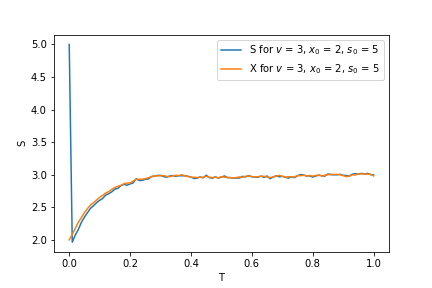
\includegraphics[scale=.6]{随机微分方程解2参数初值.png}
    \caption{参数 $v$ 和初值对随机微分方程2解的轨道影响}
    \label{fig:SDE2_x0}
    \end{figure}








\section{总结}







\bibliographystyle{plain}
\bibliography{references}
\end{document}